%%%%%%%%%%%%%%%%%%%%%%% CHAPTER - 2 %%%%%%%%%%%%%%%%%%%%\\
\chapter{Review of Related Works}
\label{Ch:Literature} %%%%%%%%%%%%%%%%%%%%%%%%%%%%
\graphicspath{{Figures/chapter2-Lit/}}

\section{Introduction}


This chapter describes various aspects in the  development of an \gls{asr} system for Malayalam language. It starts with a comprehensive review of different speech recognition architectures in Section \ref{sec:Literature-architecture}, which helps to make an informed choice of the right architecture for building the Malayalam ASR system. 
% We justify the selection of a hybrid \gls{dnn}-\gls{hmm}  architecture in Section \ref{sec:Literature-architecture}. 

One of the critical components of building an ASR system is the \gls{g2p} conversion system. In Section \ref{sec:Literature-g2p}, we discuss the need for \gls{g2p} conversion systems and the various approaches we can take to build them. G2P conversion systems are crucial in transforming the words into sequence of fundamental speech units (phonemes), which is essential in developing an ASR system. Additionally, we also explore the creation of ready to use \acrfull{pl} for different languages in Section \ref{sec:Literature-pl}. A \gls{pl} is a dictionary that contains a mapping of words to their corresponding phonemes. These pre-built lexicons can aid in building an ASR system more efficiently and accurately. We then move on to discuss how the morphological complexity of languages is quantitatively analysed in Section \ref{sec:Literaure-morphcomplexity}. As we explore the Malayalam language, we find that it has a high degree of morphological complexity, which presents some unique challenges for developing an ASR system. We explain how we can overcome these challenges and the approaches we can take to tackle them.

As we move on to discuss the development of ASR systems in languages with high morphological complexity in Section \ref{sec:Literature-morphasr}, we explore some of the challenges faced in developing these systems. We look at some of the approaches and techniques that researchers have used to address these challenges and to build effective ASR systems for such languages. Then in section \ref{sec:Literature-corpora}, we document various openly available speech and text corpora available in Malayalam for developing speech and language technology applications. Finally, we review previous reported works on the development of ASR systems for the Malayalam language in Section \ref{sec:Literature-malayalamasr}. We examine the different approaches taken by researchers and the outcomes of their efforts in building ASR systems for Malayalam. This review will help to understand the progress made in this field and the areas that require further attention in developing an effective ASR system for Malayalam.


% This chapter presents the various aspects of developing an \gls{asr} system
% for the Malayalam language.  A review of
% different speech recognition architectures is given, and the choice of a hybrid
% \gls{dnn}-\gls{hmm} architecture for building the Malayalam \gls{asr} system is
% justified in section \ref{sec:Literature-architecture}. Then we discuss how morphological complexity of
% languages are quantitatively analysed in Section
% \ref{sec:Literaure-morphcomplexity}. In section \ref{sec:Literature-g2p}, the
% need for \gls{g2p} conversion systems and the various approaches to build
% them is discussed.
% % The creation of pre-built \gls{pl} for different languages is discussed in section \ref{sec:Literature-pl}.   
% The development of \gls{asr} systems in languages with high morphological
% complexity is covered in section \ref{sec:Literature-morphasr}. Finally, previous works
% on the development of ASR systems for the Malayalam language are discussed in
% section \ref{sec:Literature-malayalamasr}.

% This chapter discusses various aspects of the development of an \gls{asr} system for Malayalam language. We present an overview of various speech recognition architectures and provide a justification of our choice of hybrid \gls{dnn}-\gls{hmm} architecture to build Malayalam \gls{asr} system in \ref{sec:Literature-architecture}. Then we present the need for \gls{g2p} conversion systems and the different approaches in building them in \ref{sec:Literature-g2p}. It is followed by a discussion on how ready to use \gls{pl} is built for different languages in \ref{sec:Literature-pl}. Then we discuss how morphological complexity of languages are quantitatively analysed in \ref{sec:Literaure-morphcomplexity}. After that, in \ref{sec:Literature-morphasr}, we present the development of \gls{asr} systems in lanaguages of high morphological complexity. It is followed by a discussion on various previous works on the development of \gls{asr} systems in Malayalam language in \ref{sec:Literature-malayalamasr}. 
\section{ASR System Architectures} \label{sec:Literature-architecture}

The development of \gls{asr} architectures has undergone significant changes since its inception in the mid-twentieth century. One of the early attempt of \gls{asr} was the basic word template matching method, which was used for isolated digit recognition in English in 1952 \cite{davis1952automatic}. The Harpy system  \cite{lowerre1976harpy}  introduced in 1972, used phoneme level template matching and graph based search for recognising spoken sentences with a limited vocabulary. However, a major breakthrough in ASR research occurred in the 1990s with the release of open source \gls{hmm} toolkits such as HTK \cite{young2002htk} CMU Sphinx \cite{lee1990overview} and Kaldi \cite{povey2011kaldi}.

These toolkits effectively combined the concepts of \gls{hmm}, \gls{gmm}, and statistical language models, which had been introduced in the 1970s and 1980s \cite{meyer2019multi}. This led to the development of more accurate and robust ASR systems capable of recognising larger vocabularies and handling variations in speech due to factors such as accent and speaking rate. Recent advancements in deep learning techniques such as Transformer models have further improved the performance of ASR systems, leading to their widespread use in various applications such as virtual assistants, transcription services, and language translation.

In the following sections we describe in detail the pipeline architecture of \gls{asr} and an overview of \gls{e2e} \gls{asr} architecture.

% \Gls{asr} architectures have undergone huge changes since its inception in the middle of twentieth century \cite{meyer2019multi}. The earliest attempt of basic word template matching method  for isolated digit recognition in English was reported in 1952 and the Harpy system that used phoneme level template matching and graph based search for recognising spoken sentences with a limited vocabulary  was reported in 1972. A major breakthrough in the \gls{asr} research domain happened with the release of the open source \gls{htk}  and CMU Sphinx  toolkits in 1990s. These toolkits effectively combines the concepts of \gls{hmm}, \gls{gmm} and the statistical language model introduced in 1970s and 1980s 
\subsection{Pipeline Architecture}

\begin{figure}[ht]
	\begin{center}
		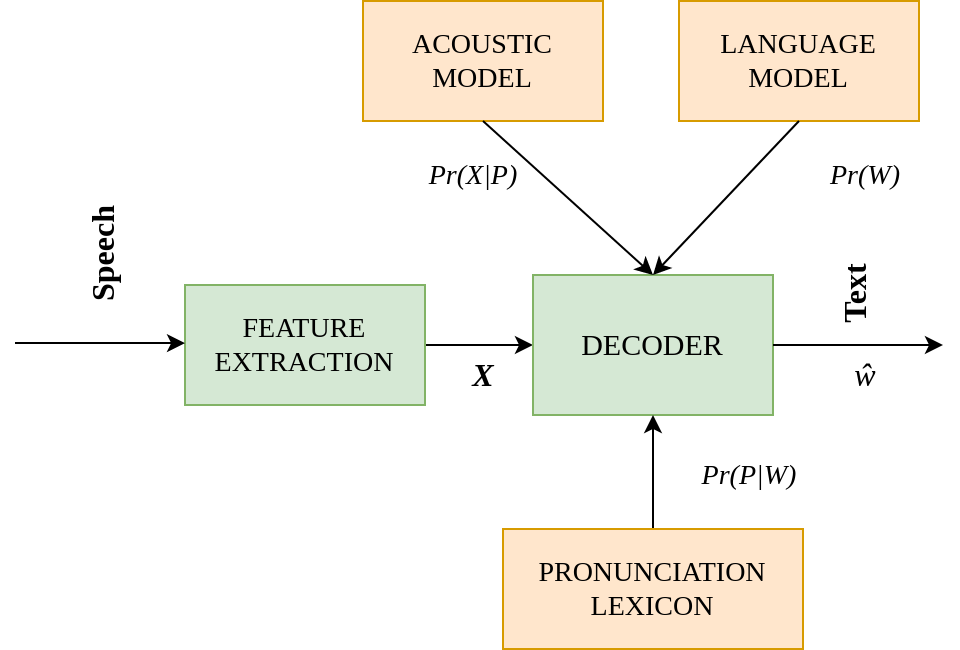
\includegraphics[width=0.7\linewidth]{asr-decoder.png}
		\caption{Architecture of a pipeline ASR  decoder}
		\label{fig:asr-decoder}
	\end{center}
\end{figure}

We present the most widely used \gls{asr} architecture here. A pipeline ASR is built on different
components, each one developed independently during the training stage.  The
components are: an \gls{am} typically implemented using a statistical approach or using a neural network, a static
\gls{pl}, and a \gls{lm} usually represented as a probabilistic
component. The decoding process is carried out using a \gls{wfst} which is
created by combining these elements through composition operations
\cite{gales2008application}. This
pipeline structure shown in Fig. \ref{fig:asr-decoder} \cite{georgescu2021performance} is now considered the classical architecture with the advent of modern
\gls{e2e} ASR architectures. In this figure, \gls{Probability} indicates the probability function, \gls{X} indicates the speech feature vector, \gls{P} indicates the phonemes, \gls{W} indicates the words in a sentence and \gls{Wcap} indicates the words predicted by the \gls{asr} decoder. The steps in pipeline architecture of ASR are described in the following subsections.



\subsubsection{Feature Extraction}

The waveform of raw speech signal in a speech corpus is simply a representation of air
pressure variation over time. In order to extract information that is relevant
for acoustic modelling, the raw speech signal is transformed into alternate
representations. This process involves splitting the audio into frames of fixed
size using overlapping windows. The window shapes, like Hamming or Hanning, are
designed to smoothen frame border discontinuities in order to avoid the
occurrence of frequency artifacts \cite{oppenheim1999discrete}. Typically the
window size is 25ms with 10ms overlap with previous frame. The series of
frequency domain transformations on each frame returns a low dimensional
feature vector \cite{meyer2019multi}.

\begin{figure}[ht]
	\begin{center}
		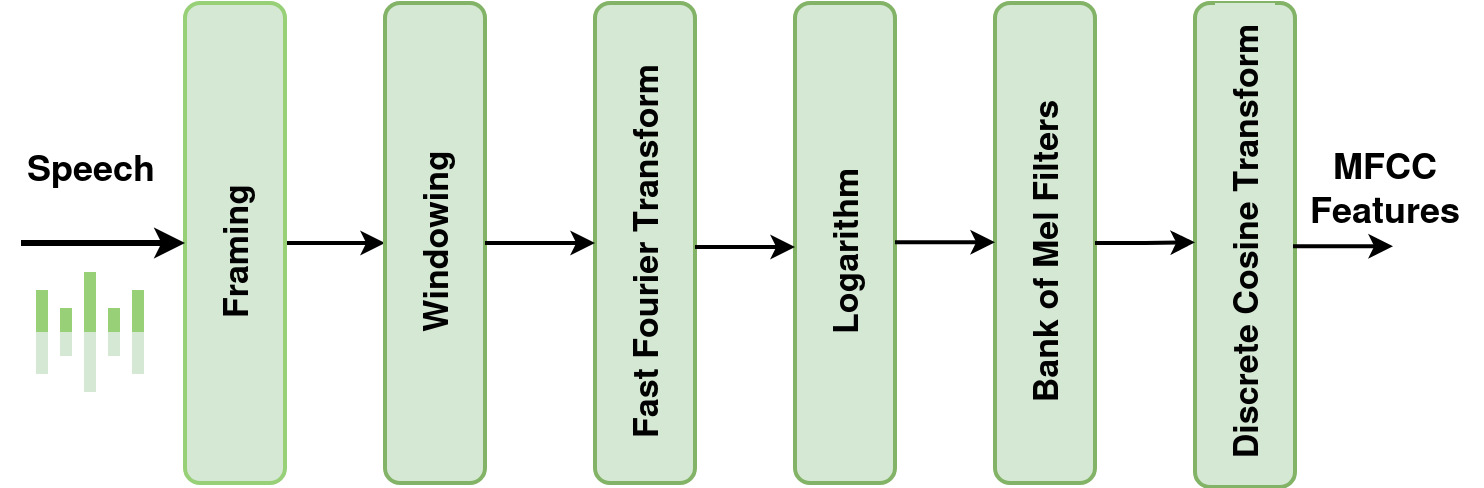
\includegraphics[width=0.9\linewidth]{featureextraction.jpg}
		\caption{Extracting Speech Features}
		\label{fig:feature-extraction}
	\end{center}
\end{figure}


\Gls{mfcc} is one of the most popular acoustic feature used in speech recognition systems. The extraction of this feature is described in Fig. \ref{fig:feature-extraction} \cite{georgescu2021performance}. Alternately, there are features like \gls{lfbe}, or \gls{plp} cepstral coefficients that provide good acoustic
representations of speech units (or phones) while suppressing variations in the
signal due to factors such as the speaker, channel, speaking style, and
recording environment \cite{madhavaraj2020strategies}. In all our experiments,
we have used MFCC features unless stated otherwise. In addition to the \gls{mfcc}s, first-order
(delta) and second-order (delta–delta) regression coefficients are often appended in a heuristic attempt to
compensate for the conditional independence assumption made by the HMM-based acoustic models \cite{benesty2008springer}. For DNN based acoustic
modelling we have additionally used i-vectors as feature vectors \cite{saon2013speaker}. 


\subsubsection{Acoustic Model (GMM-HMM)}

A phoneme is the fundamental unit of speech in a language. To create an \gls{am}, each phoneme in a 
language is given an identifiable label. The \gls{am} represents the
relation between the phoneme labels and the acoustic features
\cite{madhavaraj2020strategies}. The acoustic manifestation of a phoneme is
dependent on the speaker, rate of speech delivery, environmental factors and
additionally on the phoneme context in which it occurs. To model the temporal variations of a phoneme we use \gls{hmm} with
multiple states. It allows for fine grained modelling of a single phoneme into its component parts. 

When a single independent phoneme is modelled using an HMM, we call that the monophone acoustic modelling scheme. However the acoustic realisation of the
phoneme depends largely on the context of its occurrence. A vowel occurring in 
between two plosives behave differently to that of a vowel that occurs at the
beginning of an utterance. When a phoneme in different contexts is modelled using different HMMs the modelling effectiveness would be better. This type of an acoustic model which
takes into account the left and right context of a phoneme is called the
triphone acoustic model. In triphone acoustic model, the speech units are labelled as triphones. The HMM states of triphones having similar acoustic identities are given same labels and are called tied states. The similar sounding triphone states that are tied together are determined by phonetic decision trees \cite{young1994tree}.




% \begin{enumerate}
% \item a set of states 
% \item a set of transitions between states
% \item  transition probability: the probability of traversing each transition
% \item a set of possible observations
% \item emission probability: probability of each state generating each possible observation 
% \end{enumerate}


\begin{figure}[ht]
	\begin{center}
		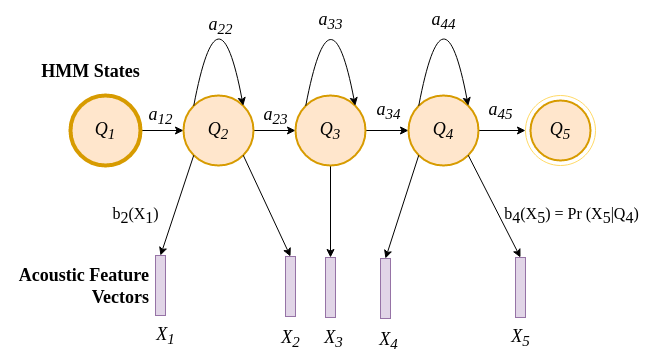
\includegraphics[width=0.8\linewidth]{gmm-hmm.png}
		\caption{GMM-HMM model of a phoneme, $P$}
		\label{fig:gmm-hmm}
	\end{center}
\end{figure}

In general an \gls{hmm} is defined by: 
\begin{enumerate}
    \item  a set of states, \gls{Q} $= \{Q_0, Q_1, ... Q_N\}$
    \item a set of transitions between states
    \item  transition probability, \gls{transition}: the
probability of traversing from state \gls{Qi} to $Q_j$
    \item a set of possible observations which are acoustic (speech) feature vectors, $X_k$
    \item  observation probability, \gls{observationprobability}: probability of state $Q_i$ generating  possible observation $X_k$.
\end{enumerate}
While modelling a phoneme using \gls{hmm}, the acoustic features, $X_k$ are the
observations. The set of hidden states are referred to as senones. Each phoneme is composed of multiple senone states indicated by $Q_i$. Each state
in an \gls{hmm} is defined by an observation probability density function specified by
multivariate Gaussians or \gls{gmm}s indicated by $\mathcal{N}(\mu,\sigma^2)$, where $\mu$ and $\sigma^2$ indicate the mean and variance of the observations \cite{gales2008application}. These Gaussians represent the probability of audio feature vectors, \gls{Xk} given the phoneme state label $Q_i$, ie., $Pr(X_k|Q_i)$. The
transition between states are strictly left to right with the addition of self
loops. This ensures a phoneme can always be represented by the same GMM-HMM
model, whether it is uttered fast or slow. A slowly uttered phoneme will pass
through more self loops. This structure of GMM-HMM phoneme model is
described in Fig. \ref{fig:gmm-hmm} \cite{meyer2019multi,benesty2008springer}. The purpose of GMM-HMM acoustic model training is to estimate the parameters of
this model, corresponding to every phoneme. These parameters are learnt from a
huge collection of speech, spoken by multiple speakers.

\subsubsection{Acoustic Model (DNN-HMM)}

Instead of using \gls{gmm}s to model the observation probability density function
of the \gls{hmm} states, \gls{dnn}s \cite{hinton2012deep} can as well be used. This
configuration as shown in Fig. \ref{fig:dnn-hmm} is referred to as the hybrid DNN-HMM acoustic model \cite{meyer2019multi,yu2015deep}. The \gls{dnn}s have the audio frame features at the input and \gls{hmm} state labels
at the output. The DNN model training procedure relies on the \gls{gmm}-\gls{hmm} training to produce labelled data.  The
advantage of using DNNs instead of GMMs is that they are better equipped to
learn complex non-linear functions \cite{madhavaraj2020strategies}. 


\begin{figure}[htpb]
	\begin{center}
		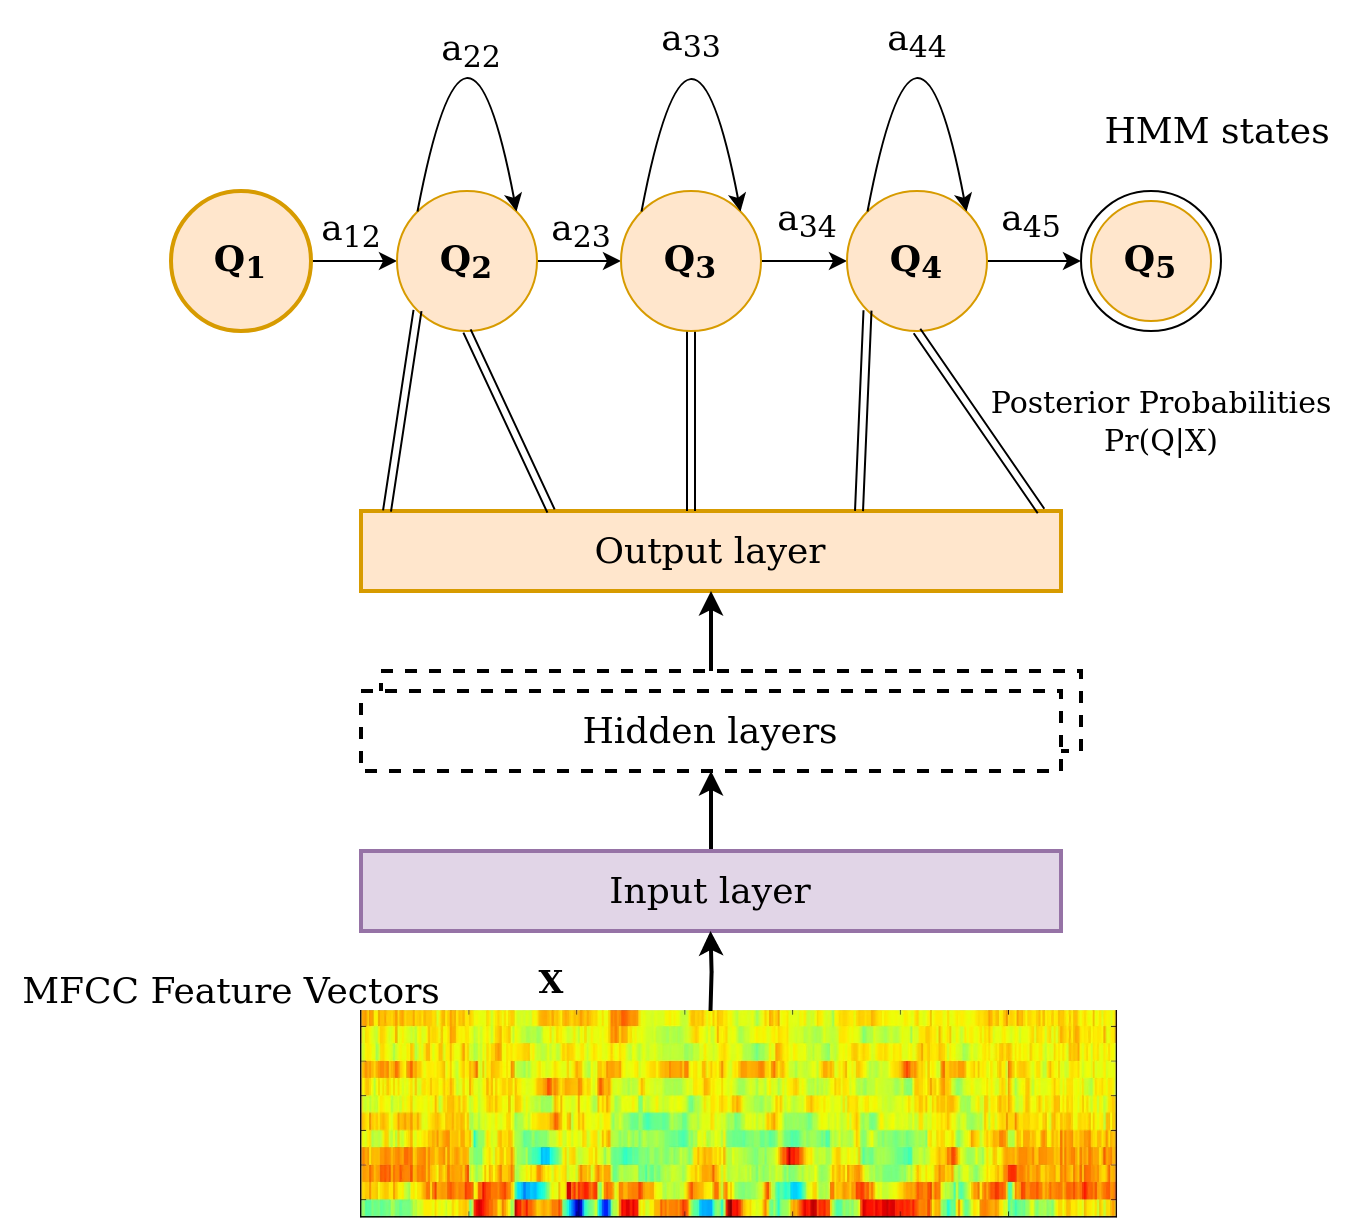
\includegraphics[width=0.8\textwidth]{dnn-hmm.png}
		\caption{DNN-HMM model of a phoneme, $P$}
		\label{fig:dnn-hmm}
	\end{center}
\end{figure}

Even though the labels come directly from the GMM model, for the DNN, each
training data instance (audio feature vector) will contain additional contextual
information about the left and right frames \cite{meyer2019multi,yu2015deep}. Unlike
GMM-HMM models which predict the likelihood of audio feature vector given a context dependent phoneme state, hybrid
DNN-HMM models predict the posterior probability of a  context dependent tied phoneme state given an audio, $Pr(Q|X)$.
However both defines a relation between audio and phonemes. 

The GMM-HMM training is called generative training while the DNN-HMM is called
discriminative training. In discriminative training, models are trained to to
maximise the separation between the correct and incorrect labels, or to
discriminate between correct and incorrect labels rather than simply assign
high weights to the correct sequence of
labels\footnote{\url{https://m-wiesner.github.io/LF-MMI/}}. The discriminative training objective is usually based on reducing the frame level cross-entropy loss as in equation \ref{eq:trainingcriteria}, where ${Q}$ and \gls{Qcap} represents the true and predicted HMM state labels.

\begin{equation}
    \label{eq:trainingcriteria}
	L_{CE}(Q,\widehat{Q}) = \sum_{i=1} Q_i \log(\frac{1}{\widehat{Q}_i})
\end{equation}

An improvement over the basic feed forward DNN to use more temporal context would be to use \gls{tdnn} as demonstrated in Fig. \ref{fig:tdnn} \cite{peddinti2015time}. Each layer in \gls{tdnn} acts at different temporal resolution, where higher layer are designed to have a wider receptive field. 
% \gls{tdnn} in acoustic modelling can be considered as a 1-D \gls{cnn}.
Since there would be overlap between input contexts at adjacent time steps, the connections in the network are sub-sampled as shown by solid lines in Fig. \ref{fig:tdnn}. It reduces redundancy and improves computational efficiency during training.


\begin{figure}[ht]
	\begin{center}
		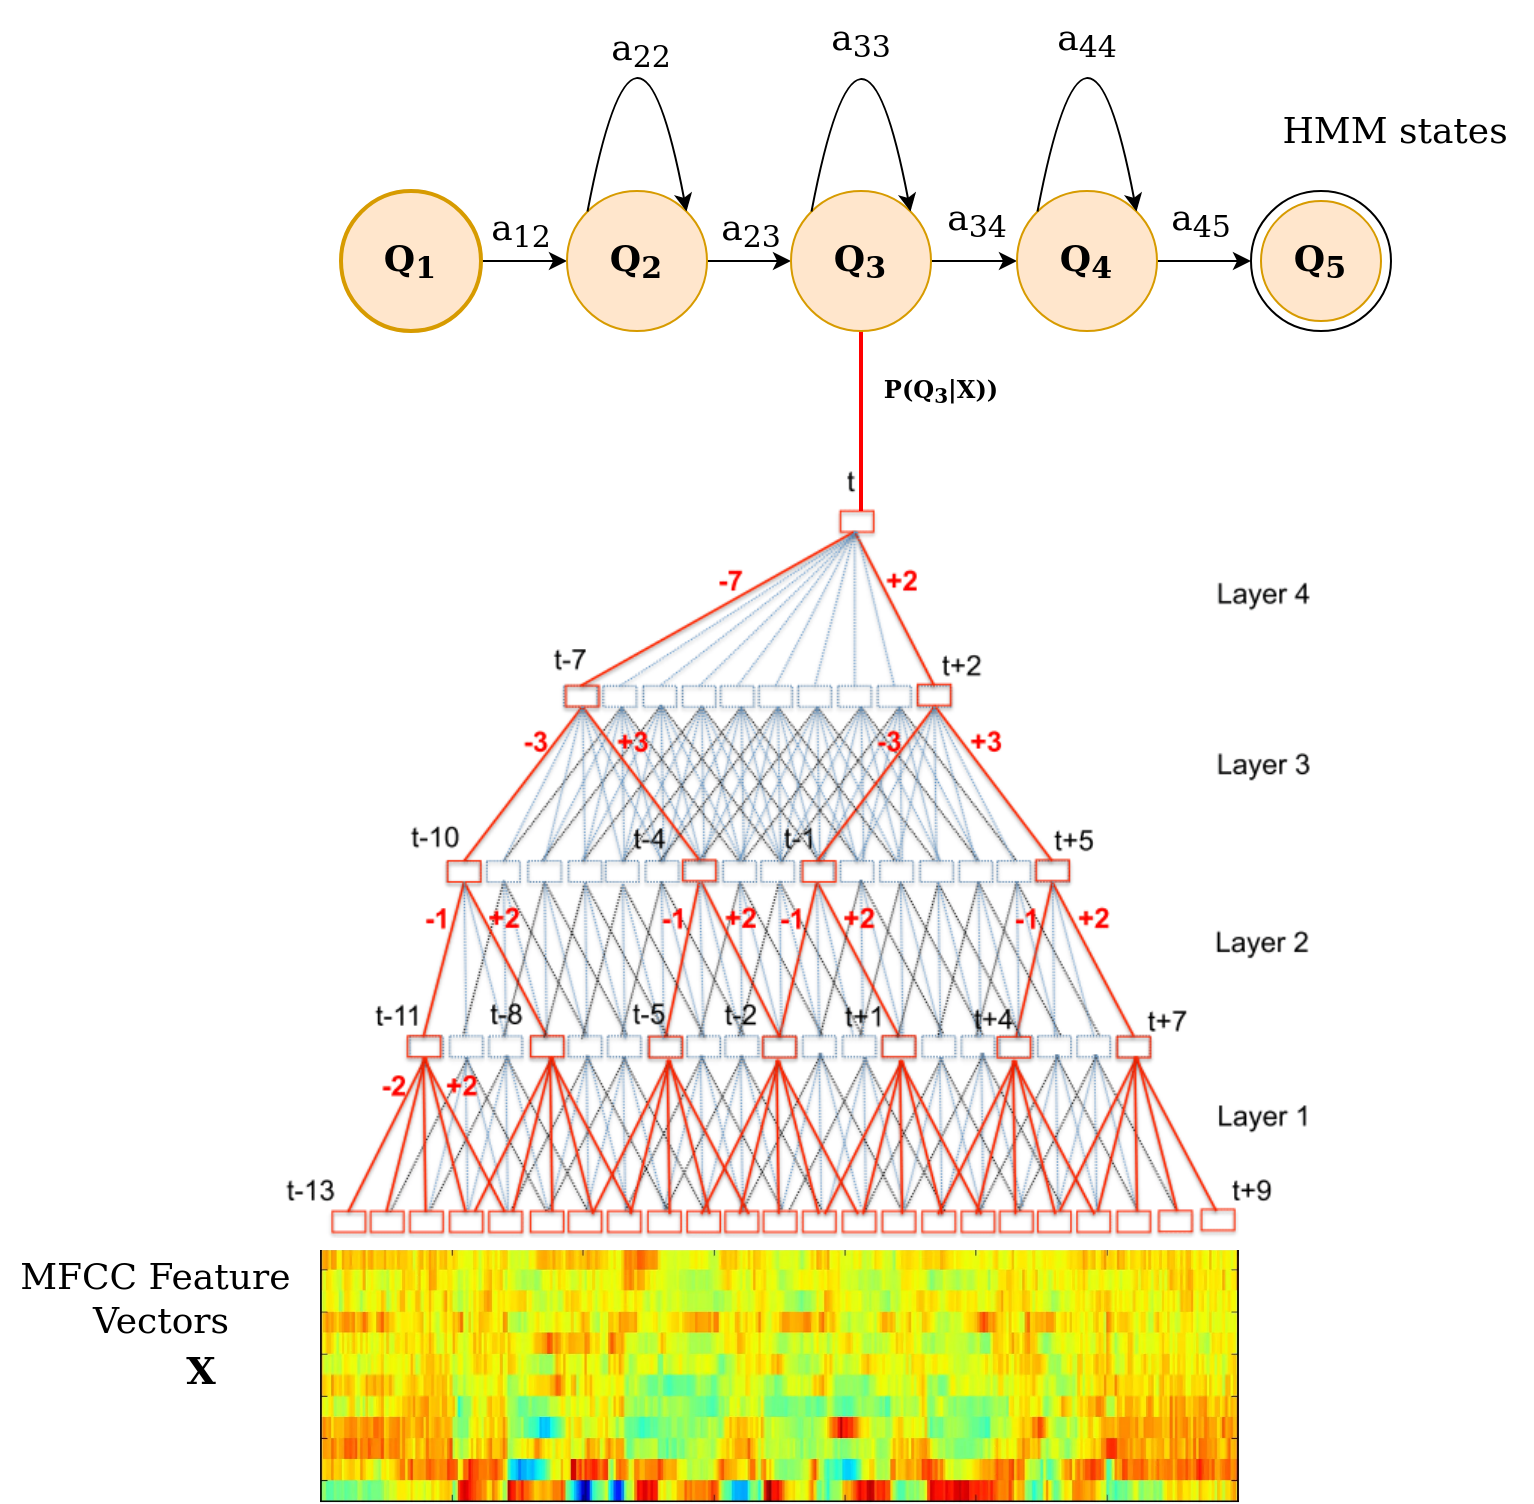
\includegraphics[width=0.8\textwidth]{tdnn.png}
		\caption{TDNN based acoustic modelling with sub-sampling (red) and without sub-sampling (blue+red).}
		\label{fig:tdnn}
	\end{center}
\end{figure}



A factored form of TDNNs (TDNN-F) which is structurally the same as a TDNN whose layers have been compressed via singular value decomposition, but is trained from a random start with one of the two factors of each matrix constrained to be semi-orthogonal has proven to give substantial improvements over TDNNs \cite{povey18_interspeech}. 


Hybrid DNN-HMM architectures using frame level cross entropy loss as a
discriminative training criteria can be aided by \gls{mmi} objective.
The \gls{mmi} training objective tries to predict the correct sequence of words
corresponding to an utterance as a whole \cite{vesely2013sequence}. The
\gls{lfmmi} algorithm proposed in \cite{povey2016purely}, has enabled the usage
of GPUs to implement the \gls{mmi} criteria and has reported improved ASR
results. The Kaldi implementation of TDNN-F has been the choice of DNN-HMM acoustic model in the current research, due to its proven acoustic modelling efficiency in the context of limited training data.


\subsubsection{Pronunciation Lexicon}

% \gls{pl} is a lookup table, which maps every word or subword to its pronunciation described as a sequence of phonemes. The lexicon model serves as a link between the acoustic and language models. The pronunciations of Malayalam is mostly one-to-one with some exceptions. These exception rules are handled using the bidirectional \gls{g2p} toolkit which can automatically generate pronunciation lexicons. This toolkit we developed is explained in Chapter \ref{ch:Mlphon}.  If a particular word has more than one pronunciations, we have added alternate pronunciations as well. While generating \gls{pl} of subwords, which do not have a valid pronunciation, we have used graphemic \gls{pl}.

A \acrfull{pl} is an important component in speech recognition and synthesis systems. It serves as a mapping between written words and their corresponding pronunciations, usually represented as a sequence of phonemes. In a classical \gls{asr} system, the acoustic model undergoes training using annotated speech corpora, where the annotations consist of word-level transcripts of the spoken utterances. However, to align the utterances with phoneme-level transcriptions, the training process relies on the \gls{pl}. This lexicon additionally holds a crucial role within the \gls{asr} decoder, working in tandem with the acoustic model and the language model to ensure precise transcription of the spoken content \cite{benesty2008springer}.

In the case of Malayalam, a \gls{pl} is used to map every word or subword to its pronunciation using a one-to-one mapping, with some exceptions that are handled using a bidirectional \gls{g2p} toolkit, Mlphon, developed as part of this research work and explained in Chapter \ref{ch:Mlphon}. The G2P toolkit is an automated system that can automatically generate pronunciations. In some cases, a word may have multiple valid pronunciations, and these alternate pronunciations are also included in the PL. This can happen for a variety of reasons, such as regional variations in pronunciation or different meanings associated with different pronunciations.

\begin{table}[h]
	\begin{center}
			\caption{A phonemic and graphemic pronunciation lexicon}
			\label{tab:pl}
			\begin{tabular}{lll}
				\hline\hline
			 Word             & Phonemic Lexicon             & Graphemic Lexicon                      \\
				\hline
				{\mal ഈ}         & {\ipa iː}                               & {\mal ഇ ൗ}                 \\
				 {\mal ഉന്നത}      & {\ipa u n n a t̪ a}                      & {\mal ഉ ന ് ന ത}               \\
			 {\mal  എന്ന}       & {\ipa e n̪ n̪ a }                         & {\mal എ ന ് ന}           \\
			 {\mal  ഒരു}        & {\ipa o ɾ u }                           & {\mal ഒ ര ു}                  \\
			 {\mal കഫേ}       & {\ipa k a f eː}                         & {\mal ക ഫ േ}               \\
			 {\mal ഫോട്ടോ}     & {\ipa f oː ʈ ʈ oː}                      & {\mal ഫ ോ ട ് ട ോ}                    \\
				\hline
			\end{tabular}
	\end{center}
\end{table}


Finally, when generating the PL for subwords (i.e., smaller units of language that are not complete words), sometimes a graphemic PL is used. This means that the pronunciation is based solely on the spelling of the subword and not on any specific established pronunciation. This approach can be useful for handling subwords that have ambiguous pronunciations. Example entries from a phonemic and graphemic \gls{pl} is shown in Table \ref{tab:pl}. The probability of a phoneme sequence given a word segment can be estimated from this lexicon and this probability $Pr(P|W)$ is referred to as the lexical model where $P$ indicates the phoneme  label.



\subsubsection{Language Model}

A \acrfull{lm}, predicts the most probable word (or subword) sequence, given
the list of previously occurred words or subwords. For a sentence $W$ formed by
sequence of $N$ word (or subword) segments $W = w_1,w_2$ \gls{wi} $. . . w_N$, the probability $Pr(W)$
of the sentence is given by the following formula applying the chain rule of
probability.

\begin{align}
	Pr(W) & = Pr(w_1,w_2,... w_N)                              \\
	     & = Pr(w_1)Pr(w_2|w_1)...Pr(w_N|w_{N-1},w_{N-2}...w_1)
	 % &=  P(s_1) \prod_{i = 2}^{N} P(s_i |s_{i-1}s_{i-2}...s_2, s_1)
\end{align}

Based on the Markovian assumption of n-gram language modelling, probability of
each segment depends only on the previous $n-1$ segments. This makes the
sentence probability to be computed as:
\begin{align}
	Pr(W) & = \prod_{i = 1}^{N} Pr(w_i |w_{i-1},w_{i-2}..w_{i-(n-1)})
\end{align}

The probability of words (or subwords) following each other can be
calculated based on a large amount of text data. The most common n-gram models
are bigram and trigram, where the history of one or two words or subwords is
taken into account, respectively. Since $Pr(W)$ encodes information about grammatically valid sequence of segments, it is also referred to as the grammar model. Back-off probabilities are estimated using
Kneser-Ney algorithm to avoid the zero-probable word sequence problem
\cite{Kneysmoothing1995}.

\subsubsection{Decoding Graph}

The function of an \gls{asr} decoder is to find the sequence of segments which are usually words $W=w_1 ,	. . ., w_K$ that is most likely to have generated the observed feature vectors
${X}=X_1, . . . , X_T$. 

The decoder tries to find

\begin{equation}
	\widehat{W}=\argmax_W\ Pr(W|{X})
\end{equation}

By the Bayes’ rule, this equation could be transformed into an equivalent form:

\begin{align}
	\widehat{W} & = \argmax_W\ \frac{Pr({X}|W)Pr(W)}{P({X})}       \\
	            & = \argmax_W\ Pr({X}|W)Pr(W) \label{eq:decoder}
\end{align}

The feature vector probability $Pr({X})$ is independent of the word probabilities
and hence can be ignored to simplify the equation as in \ref{eq:decoder}
\cite{benesty2008springer}. The likelihood $Pr({X}|W)$ is determined by the
acoustic and phonetic models and the prior $Pr(W)$ is determined by the language model. 

The probability $Pr(X|W)$ can be further decomposed into 

\begin{align}
	 % & = Pr(X,Q,P|W)      \\
	 %        & = Pr(X|Q,P,W) Pr(Q|P,W) Pr(P|W) \\
     Pr(X|W)        & = Pr(X|P) Pr(P|W) \\
      & = Pr(X|Q) Pr(Q|P_{CD}) Pr(P_{CD}|P) Pr(P|W)
\end{align}

where $Q$, \gls{PhonemeCD} and $P$ represents the HMM states, context dependent phonemes and context independent phonemes respectively. The link between the word segments $W$ and  the context independent phonemes  $P$ is provided by the lexical model  $Pr(P|W)$, derived from  a dictionary associating each word from the language model to a sequence of phonemes as shown in Table \ref{tab:pl}. 
%modelled by the acoustic model \cite{georgescu2021performance}.



The building blocks of \gls{asr} are implemented in toolkits like Kaldi
\cite{povey2011kaldi}, in the form of \gls{wfst}s \cite{mohri-1997-finite}.
The weights in WFST can be interpreted similar to a probability. The language
models are implemented as a grammar \gls{wfst}, referred to as \texttt{G.fst} which encodes the information in $Pr(W)$.
It accepts valid sequences of words, and returns both a weight and that same
sequence of words. To encode the lexical information about word pronunciation from the
\gls{pl}, Kaldi uses a WFST called \texttt{L.fst}. This WFST accepts a sequence
of phonemes and returns a word and a weight and it is derived from the probabilities $Pr(P|W)$. The next WFST, called
\texttt{C.fst}, encodes information about the relationship between  context independent phonemes in
the lexicon and the context dependent phonemes $P_{CD}$, whose states form the HMM. The final \gls{wfst}, called
\texttt{H.fst} maps the HMM state labels to $P_{CD}$, ie., $Pr(Q|P_{CD})$
\cite{meyer2019multi}. Once the H, C, L and G WFSTs are created, they are
composed from right to left to form a single WFST, after which HMM self-loop
arcs are added to form the final \texttt{HCLG.fst} which maps state
labels to word sequences \cite{madhavaraj2020strategies,povey2012generating}. While composing,
determination and minimisation operations may also be  performed  at
intermediate stages to reduce the graph size and complexity
\cite{madhavaraj2020strategies}.
\begin{figure}[htpb]
	\begin{center}
		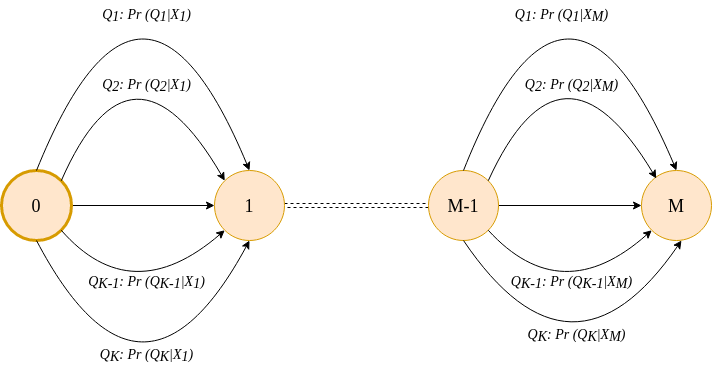
\includegraphics[width=0.8\linewidth]{acceptor.png}
		\caption{Finite state acceptor graph formed by the sequence of M feature vectors extracted from speech to be decoded}
		\label{fig:feature-fsa}
	\end{center}
\end{figure}


During the decoding phase, the acoustic feature vectors corresponding to the speech to be decoded is extracted.  If there are $M$ feature vectors, then a finite state acceptor graph with state labels $0$ to $M$ is constructed as shown in Fig. \ref{fig:feature-fsa} \cite{povey2012generating}. If there are $K$ HMM states defined in our acoustic model, then there will be $K$ possible transition paths between every state. These transition paths are given the same labels as that of the HMM states, $Q_i ; i= 1,2,..K$ and the corresponding observation probability $Pr(Q|X)$ as weights. These probability values  are obtained from GMMs or DNNs based on the type of acoustic model used. 

% we obtain the acoustic feature vector sequence of length ‘M ’ and
% create a finite state acceptor graph (A-WFST) as shown in figure 2.8, where the arcs from state
% ‘m − 1’ to state ‘m’ have PDF IDs as labels, and observation probability of the mth feature
% vector from the corresponding PDF IDs as weights. These values are obtained from GMMs or
% DNNs based on the type of acoustic model used. 

% The acoustic feature vector extracted from the speech segment to be decoded is analysed to determine the probability $Pr(Q_i|X)$, where $Q_i$ represent the label of  $i^{th}$ HMM  state. A finite state acceptor graph is constructed based on this probabilities as described in Fig. . 


This graph is composed with the ASR model graph \texttt{HCLG.fst}, to obtain a search space. A Viterbi decoding is performed on this final graph, by applying beam pruning to reduce the exponential search space \cite{benesty2008springer,jurafsky2014speech}. This returns the best decoding path and thus a decoded sequence of words.

\subsection{End to End (E2E) Architecture}
\label{sec:Literature-e2e}

Another major round of revolution in the field of \gls{asr} occurred with the advent of an
alternate approach of \acrfull{e2e} ASR. \Gls{e2e} system is a type of \gls{asr} model that
directly maps the raw audio input to the final text output, without the need
for separate acoustic, language and pronunciation modelling stages. \Gls{e2e}
models are typically trained on massive datasets (thousands of hours) which are available only to
high resource languages. This is because \gls{e2e} training techniques require thousands of hours of data to learn a
mapping of audio directly to characters without any explicit intermediate linguistic
representations. 

% \begin{figure}[ht]
% 	\begin{center}
% 		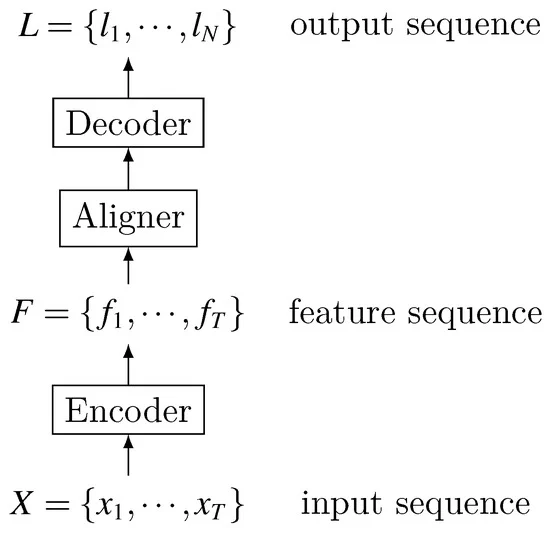
\includegraphics[scale=0.5]{e2e.png}
% 		\caption{End-to-end ASR system architecture \textit{To redraw}}
% 		\label{fig:e2e}
% 	\end{center}
% \end{figure}

The training techniques that learns sequence to sequence mapping between acoustic feature frames and character sequences has evolved a lot during the past few years \cite{prabhavalkar2023end}. There are explicit alignment approaches like \gls{ctc}  \cite{graves2006connectionist}, \gls{rnn} \cite{graves2012sequence} transducer and \gls{rna} \cite{sak2017recurrent} and implicit alignment approaches like \gls{aed} methods. In addition to the massive data requirement, the training procedure is compute-intensive with specialised hardware requirement \cite{anoop2023exploring}. 
% Unlike the hybrid approach, there is no alignment information available to train an \gls{e2e} \cite{chorowski2014end} system.

% The \gls{e2e} architecture is trained on a single objective function to predict
% the text transcript directly from the audio. It consists of an encoder, an
% aligner and a decoder as shown , in Fig. \ref{fig:e2e}. Note that all those
% modules may not always exist in the E2E framework.  The
% alignment information in E2E architectures are extracted using either (i)
% \gls{ctc} (ii) \gls{rnn} transducer and
% \cite{graves2012sequence} (iii) attention based framework
% \cite{chorowski2014end}.

For low resource languages like Malayalam, where the availability of annotated speech corpora under open licenses is limited to less than 100 hours, training an \gls{e2e} ASR from scratch is practically impossible. However there is much more text data available to train separate language models. That has motivated the researcher to stick on to the hybrid DNN-HMM architecture, where acoustic models can be trained on the available smaller corpora and leverage the language model to obtain good decoding results \cite{SMIT2021101158}. But at the time of writing this thesis, there are many pre-trained \gls{e2e} models trained using self supervised learning approach \cite{baevski2021unsupervised,radford2022robust}. They are trained on many multilingual un-annotated speech datasets, many of which are undisclosed. These pre-trained models can be fine tuned on a small annotated speech dataset, which may be a promising approach for low resource languages. 
% However this thesis does not go much into an exploration in that direction.



% \subsection{Pretrained Transformer Architectures}

% \textit{Transformer models to be discussed here}

% In order to design and develop an \gls{asr} system, huge amount of diverse language resources are needed. A parallel corpus of recorded speech and its textual transcription, text data corpus, phonetic lexicon are the three essential language resources needed for developing an \gls{asr} system. Malayalam is spoken by about 38 million native speakers in southern India. But the availability of these linguistic resources are very limited for Malayalam, making it a resource scarce language at present.


\section{Grapheme to Phoneme Conversion Systems} \label{sec:Literature-g2p}

This section focuses on a broad review on automatic \gls{g2p} conversion systems available in Malayalam and its relation with other world languages. Solutions for automatic \gls{g2p} conversion in one language may not be the
optimal solution applicable for a different language. There are problems with 
different levels of difficulty that should be solved for each language or
language family separately \cite{mdpi2022ruleg2p}. 

Malayalam is a
morphologically complex low resource language with very little transcribed
audio datasets and no openly available pronunciation lexicons.
% Morphologically complex languages with very large number of rare words are challenging for machine translation and \gls{asr} tasks due to huge \gls{oov} rate. 
%Malayalam language is known to demonstrate a high level of morphological complexity than many other Indian and European languages in terms of type-token ratio and type-token growth rate \cite{manohar_quantitative_2020,	bharadwaja2007statistical}.
% It is the proportion of words that are not present in the vocabulary and thus cannot be recognized or translated correctly.
For languages with very little transcribed audio datasets available for speech related tasks, a precise \gls{g2p} conversion can ensure better acoustic modelling, even in \gls{e2e} \cite{baevski2021unsupervised} \gls{asr} systems.

In many languages, \gls{g2p} correspondence
depends on the relative position of grapheme within a word and a syllable,
which makes syllable boundary identification  important for phoneme
level analysis. Segmenting words to syllables has got further applications in machine translation
systems and speech to text systems especially in the context of morphologically
complex languages where subword level units improve system performance
\cite{kunchukuttan2016, SMIT2021101158}. 





Various works on mapping graphemes in Malayalam to phonemes have been reported in literature. There are language-specific as well as language-independent tools. Data driven and knowledge based approaches are the two main \gls{g2p} strategies. While languages with sufficient amounts of annotated data for training primarily rely on data driven techniques, languages with well documented pronunciation rule sets use knowledge based solutions. In the former, the \gls{g2p} rules are learned directly from data, whereas in the latter, rules are constructed using linguistic expertise.
Most of the  \gls{g2p} tools in Malayalam follow rule-based rather than machine learning approaches. This is primarily due to the simplicity of rule-based approach and secondarily due to unavailability of annotated data for training. Implementation of rule-based approaches require thorough linguistic know-how.

Data driven approaches perform \gls{g2p} mapping by dictionary lookups \cite{black1998issues}, decision trees \cite{black1998issues}, conditional random fields \cite{fosler2013conditional}, pronunciation by analogy
\cite{yvon1996grapheme} or joint sequence alignments \cite{bisani2008joint}. Recently, deep learning architectures for \gls{g2p} have been developed based on \gls{rnn}s \cite{yao2015sequence}, \gls{cnn}s \cite{yolchuyeva2019grapheme} and transformers \cite{sevinj2019transformer}. Zero shot \gls{g2p}  techniques without explicit training data have been proposed, but they are based on the assumption that similar language families
use the same orthography, which is not always true \cite{li-etal-2022-zero}. Phonetisaurus \cite{novak_minematsu_hirose_2016} is a data driven tool that learns the mapping rules statistically (joint sequence models) from a training dataset and builds weighted FSTs for \gls{g2p} conversion. Malayalam does not have a good quality annotated data set for \gls{g2p} training and a Phonetisaurus model for Malayalam has not been reported yet.

For languages with regular \gls{g2p} conversion patterns, knowledge based \gls{g2p} has been reported to produce good results \cite{li-etal-2022-zero, sar2019applying}. A set of sequential rewrite rules can be used to achieve this. Agglutinative languages like Turkish \cite{oflazer2006architecture} and Amharic \cite{anberbir2011grapheme} have reported works on language specific knowledge based \gls{g2p} conversion using FST technology. Epitran  \cite{mortensen2018epitran}, an open source tool using rule based FSTs for \gls{g2p} conversion of more than 61 world languages recently added Malayalam support, with preliminary mapping between graphemes and phonemes. Hybrid approaches that applies linguistic rules on statistical \gls{g2p} mappings have been reported for Khmer language \cite{sar2019applying}.

% 





\subsection{A Review of G2P Tools in Malayalam}
\label{sec:Literature-g2preview}

% Aswathy et al. has presented a work on automatic pronunciation lexicon generation for Malayalam using basic \gls{lts} rules with an  exception dictionary\cite{aswathy2014improving}. It uses a naive Bayes classifier to identify native and English language words and use different set of \gls{lts} to perform the phoneme mapping. This is a language specific technique, which covers many allophonic variations, but misses some contextual rules for phoneme mapping. Another rule based \gls{g2p} converter for Malayalam was implemented by Sumi et al. \cite{sumi2013Rule}. This is also a language specific tool, covering only a subset of context sensitive rules. Work on keyword spotting in Malayalam by Vivek summarizes the algorithms for grapheme to phoneme conversion for Malayalam in his thesis\cite{vivek}. \Gls{fst} based \gls{g2p} mapping for code switched Malayalam-English text has been done by Sreeja et
% al.\cite{manghat2020malayalam} where English words are phoneme mapped using CMUDict \cite{lenzo2007cmu} and contextual rule based \gls{fst} was used for Malayalam text.

% % %Nisaba Brahmic library for script normalization and processing supports reversible script transliteration and validity checks on script grammar with FST backend \cite{johny-etal-2021-finite}. 
% Unified parser is a rule based multilingual tool for parsing Indian language text and converting it to a common label set of phonemes in syllabified form\cite{baby2016unified}. Language specific logic for many Indian languages have been incorporated to this tool, but all the peculiarities of Malayalam script has not been addressed for grapheme to phoneme conversion. Festvox Indic Frontend converts text in many Indian languages to phonetic pronunciations, for
% \gls{tts} systems. It uses X-SAMPA phone set for mapping graphemes to phonemes \cite{parlikar2016festvox}. This tool also supports many language specific rules, including the handling of chillus in Malayalam, but not all contextual rules.


This section focuses on \gls{g2p} tools that works for Malayalam. Being a language with regular orthography, most of the \gls{g2p} conversion tools in
Malayalam follow knowledge based approaches
\cite{duddington2012espeak,baby2016unified,parlikar2016festvox,aksharamukha,kunchukuttan2020indicnlp,manghat2020malayalam,aswathy2014improving}
rather than data driven methods.
% This is primarily due to the availability of deterministic rules sets and secondarily due to unavailability of annotated data for training. 
The only data driven method is based on encoder-decoder architecture \cite{Priyamvada_2021} and uses data prepared using an existing knowledge based
solution, Unified Parser. Table \ref{tab:g2ptools} compares the functionalities of different
grapheme-phoneme conversion tools available for Malayalam. Here, we examine
each of their features and drawbacks in detail.

\begin{table}[htpb]
	\begin{center}
		\begin{minipage}{280pt}
			\caption{Comparing the functionalities and features of G2P conversion tools in Malayalam}
			\label{tab:g2ptools}
			\begin{tabular}{@{}lccccccccc@{}}
				\\ \hline \hline
				Tools                                     & \rotatebox{90}{Script Grammar Check} & \rotatebox{90}{Orthographic Syllabification} & \rotatebox{90}{Grapheme to Phoneme} & \rotatebox{90}{Phoneme Delimiter} & \rotatebox{90}{Phoneme Syllabification} & \rotatebox{90}{Phoneme to Grapheme} & \rotatebox{90}{Phonetic Feature Analysis} & \rotatebox{90}{Open source} & \rotatebox{90}{Programmable API} \\
				\hline
				Unified Parser  \cite{baby2016unified}    &                                      &                                              & {\tick ✓}                           & {\tick ✓}                         & {\tick ✓}                               &                                     &                                           & {\tick ✓}                   &                                  \\
				Espeak  \cite{duddington2012espeak}       &                                      &                                              & {\tick ✓}                           & {\tick ✓}                         & {\tick ✓}                               &                                     &                                           & {\tick ✓}                   & {\tick ✓}                        \\
				Festvox \cite{parlikar2016festvox}        &                                      &                                              & {\tick ✓}                           & {\tick ✓}                         & {\tick ✓}                               &                                     &                                           & {\tick ✓}                                                      \\

				Aksharamukha\cite{aksharamukha}           &                                      &                                              & {\tick ✓}                           &                                   &                                         & {\tick ✓}                           &                                           & {\tick ✓}                   &
				{\tick ✓}                                                                                                                                                                                                                                                                                                                                                                                              \\ Indic NLP \cite{kunchukuttan2020indicnlp} &  & {\tick ✓} & {\tick ✓}
				                                          &                                      &                                              &                                     &                                   & {\tick ✓}                               & {\tick ✓}                                                                                                                                        \\
				% Epritan \cite{mortensen2018epitran}                     &      &{\tick ✓}  & {\tick ✓} &         &         &           &       &{\tick ✓}\\
				Code-switched \cite{manghat2020malayalam} &                                      &                                              & {\tick ✓}                           & {\tick ✓}                         &                                         &                                     &                                           &                                                                \\
				LTS \cite{aswathy2014improving}           &                                      &                                              & {\tick ✓}                           & {\tick ✓}                         &                                         &                                     &                                           &                             &                                  \\

				Encoder-Decoder \cite{Priyamvada_2021}    &                                      &                                              & {\tick ✓}                           & {\tick ✓}                         &                                         &                                     &                                           &                                                                \\
				\hline \textbf{Mlphon}                    & {\tick ✓}                            & {\tick ✓}                                    & {\tick ✓}                           & {\tick ✓}                         & {\tick
				✓}                                        & {\tick ✓}                            & {\tick ✓}                                    & {\tick ✓}                           & {\tick ✓}                                                                                                                                                                                                                      \\

				\hline
			\end{tabular}
		\end{minipage}
	\end{center}
\end{table}

\begin{itemize}
	\item Unified parser \cite{baby2016unified} is a multi-lingual open source tool for
	      parsing Indian languages and converting it to a common label set of phonemes in
	      syllabified form. In its language-specific logic, it doesn't take into account
	      any of the Malayalam pronunciation modification rules other than the addition
	      of inherent vowels. This tool does not perform  grapheme level syllabification .
	\item Espeak \cite{duddington2012espeak} is an open source speech synthesis system
	      that has a \gls{g2p} module and it supports Malayalam. Even though phoneme
	      syllabification is supported by Espeak, it does not syllabify graphemes.
	\item Festvox Indic frontend perform  \gls{g2p}, for TTS systems. It uses X-SAMPA phone set
	      \cite{parlikar2016festvox}. On analysing the transcription it provides, many
	      contextual rules are observed to be missing for Malayalam and it does not
	      support syllabification of graphemes.
	      % This tool also supports many language specific rules, but not all. 
	\item Aksharamukha \cite{aksharamukha} script converter is an open source tool that
	      supports  \gls{g2p} for many languages. However language specific contextual logic is
	      lacking for Malayalam. It can not be used to create a pronunciation lexicon, as
	      it does not provide delimiters between phonemes. It syllabifies neither
	      graphemes nor phonemes.
	      % \footnote{Espeak TTS: \url{http://espeak.sourceforge.net/}}.
	\item The Indic NLP library \cite{kunchukuttan2020indicnlp}, supports syllabification of graphemes and performs  \gls{g2p}. This tool lacks delimiters between phonemes, so 
	      it cannot be used to create a pronunciation lexicon. 
       \item FST based  \gls{g2p}
	      mapping for code switched Malayalam-English text has been reported in
	      \cite{manghat2020malayalam}, where English words are phoneme mapped using
	      CMUDict\footnote{CMUDict- The CMU Pronouncing Dictionary:
		      \url{http://www.speech.cs.cmu.edu/cgi-bin/cmudict}} and contextual rule based
	      FST was used for Malayalam. This tool is not open source and hence not freely
	      available for further use, research or analysis. 
       \item Using basic letter to
	      sound (LTS) rules, an automatic pronunciation lexicon creation work was
	      proposed in \cite{aswathy2014improving}. It uses a naive Bayes classifier to
	      identify native and English language words and use different set of LTS to
	      perform the  \gls{g2p} mapping. This tool is not openly available for further research
	      and analysis.
	\item The only deep learning based data driven approach for Malayalam  \gls{g2p} conversion
	      uses Unified Parser for creating the data set for training and testing the
	      model \cite{Priyamvada_2021}. It has the same features and shortcomings as the
	      Unified Parser tool.
\end{itemize}

%  However these tools for Malayalam are restrictively licensed and not openly available for testing.
Based on our detailed analysis of the available tools cited above, it was found
that none of these tools have full coverage of pronounceable characters defined
in Malayalam Unicode. None of these tools could handle the overloading of the
letters {\mal ഫ }(labiodental fricative and and also as labial aspirated
plosive) {\mal ന }(dental nasal and also as alveolar nasal) and their
disambiguation. Each of these tools follow different choice of phonetic
alphabets and mapping criteria, making them incompatible for a meaningful
comparison.

\subsection{Ready to Use Pronunciation Lexicon}
\label{sec:Literature-pl}

Availability of a ready to use phonetic lexicon is an essential linguistic
resource for \gls{asr} and \gls{tts} tasks.
CMUDict\footnote{\url{http://www.speech.cs.cmu.edu/cgi-bin/cmudict}} is an
open source machine readable pronunciation dictionary for North American
English that contains over 134,000 words and their
pronunciations\cite{lenzo2007cmu}. Similar efforts for creating pronunciation
dictionaries for different world languages are reported in literature, namely;
Globalphone, providing pronunciation dictionary of 20 world
languages\cite{schultz-schlippe-2014-globalphone}, The LC-STAR phonetic lexica
of 13 different languages\cite{castell2004lc}, Arabic speech recognition
pronunciation dictionary with two million pronunciation entries for 526,000
modern standard Arabic words\cite{ali2017}, ASR oriented Indian English
pronunciation dictionary\cite{huang-etal-2020-construction}, manually curated
Bangla phonetic lexicon of 65k lexical entries prepared for TTS
\cite{ttsbangla} are to mention a few.

However openly available large vocabulary pronunciation lexicon has not been
reported for Malayalam, till date. The reported works on Malayalam
pronunciation lexicons has mostly been done manually or semi-automatically with
a small or medium vocabulary for \gls{asr} tasks \cite{cinikurian,deekshitha}.
Agricultural speech and text corpora for Malayalam with 4k manually transcribed
phonetic lexicon entries has been reported by Lekshmi et al.
\cite{k-r-etal-2020-malayalam}. Considering the agglutinative nature of
Malayalam language and its practically infinite vocabulary, a manually curated,
small sized pronunciation lexicon would be inadequate for general domain speech
tasks \cite{manohar_quantitative_2020}. Also there could be need for expanding
the vocabulary of lexicon as new words get added to the language in the form of
proper nouns and loan words. Such lexicons, if available can serve as high quality annotated
data sets for bootstrapping data driven  \gls{g2p} training.


\section{Morphological Complexity Analysis}
\label{sec:Literaure-morphcomplexity}

In linguistic research, measuring the morphological complexity of a language  is a crucial area of investigation. Morphology refers to the study of the structure of words, including the formation of words and their grammatical endings, prefixes, and suffixes. The complexity of a language's morphology can be measured by analysing the number and type of morphemes present in its words and examining how they interact with one another to form meaning \cite{bane2008quantifying}. The study of morphological complexity is significant because it sheds light on how languages differ from one another and helps us understand the cognitive demands involved in using different languages. Morphological complexity of a language has its impact on applications like \gls{asr} where speech to text conversion depends largely on the underlying language model. A measure of the complexity is important for improving and adapting the existing methods of \gls{nlp}\cite{gutierrez2018comparing}. In this section we discuss what are the different techniques by which morphological complexity are quantified and how are they related.

Morphological complexity can be measured either in terms of the average number of grammatical features getting encoded into a word or in terms of the diversity of word forms occurring in the text corpus of a language. The former approach is called typological analysis and the latter one is called corpus based analysis of morphological complexity \cite{bentz2016comparison}. The number of possible inflection points in a typical sentence, the number of
inflectional categories, and the number of morpheme types are all morphological
complexity indicators \cite{bane2008quantifying}. It requires a strict linguistic supervision to analyse each word in terms of its morpheme types to quantify complexity in this manner. The work in \cite{gutierrez2018comparing} suggested estimating the morphological complexity of a language directly from the diverse wordforms over a corpus, which is a relatively easy and reproducible way to quantify complexity without the strict need for linguistic annotated data. A study was conducted to analyse morphological complexity using both human expert judgement and corpus based analysis \cite{bentz2016comparison}. Its findings revealed a strong correlation between the two approaches.

% Complexity of a natural language can be in terms of morphology, phonology or
% syntax \cite{baerman2015understanding}. Morphological level complexity of a
% language implies a large possibility of inflections (by grammatical tense,
% mood, aspect and case forms) and agglutinations (of different wordforms). 




%  A study by Kettunen suggest the usage of a text corpus based parameter \gls{ttr} and \gls{mattr} to quantitatively represent the morphological complexity of a language by analysing and comparing various European languages
% \cite{kettunen2014can}. Covington et al. suggested the use of \gls{mattr} as a reliable measure of linguistic complexity independent of the total corpus length and suggested an efficient algorithm for computing \gls{mattr} \cite{covington2010cutting}. Kettunen \cite{kettunen2014can} compared corpus based parameters like TTR and MATTR with other methods of complexity measures as defined by Patrick Juola \cite{juola1998measuring} and concluded both TTR and MATTR give a reliable approximation of the morphological complexity of languages. Ximena
% Gutierrez-Vasques et al. suggested estimating the morphological complexity of a
% language directly from the diverse wordforms over a corpus is relatively easy
% and reproducible way to quantify complexity without the strict need of
% linguistic annotated data \cite{gutierrez2018comparing}. 

Various approaches have been proposed to quantitatively represent the morphological complexity of a language. One such approach, proposed in \cite{kettunen2014can}, involves using a text corpus based parameter, namely, \gls{ttr} and \gls{mattr}, to analyse and compare various European languages. According to the work in  \cite{covington2010cutting}, \gls{mattr} is a reliable measure of linguistic complexity, independent of the total corpus length. Moreover, \cite{kettunen2014can} compared corpus based parameters such as \gls{ttr} and \gls{mattr} with other methods of complexity measures and concluded that both parameters provide a reliable approximation of the morphological complexity of languages. In current research, we rely on the corpus based parameters of \gls{ttr} and \gls{mattr} to quantitatively analyse morphological complexity of Malayalam.

% An DNN/HMM hybrid ASR system requires the graphemes to be represented as a sequence of phonemes in the pronunciation lexicon with delimiters in between. The Unified Parser, Indic Front end and Espeak provides lexicon in this format. Only Espeak implements the most common digression in Malayalam g2p mapping, the contextual substitutions needed in alveolar nasal/plosive conjuncts.

%  \item 

% Even though Unified Parser and Indic Front end provides syllabification (delimiter between syllables in the phonemized text), they do not syllabify the native script. So a syllable level mapping between graphemes and phonemes is can not be provided by these tools. Aksharamukha provides bidirectional conversion between graphemes and phonemes, but syllabify neither native script nor phonemes. Indic NLP library is an open source python library that provides syllabification of native script, but does not provide phonemes with delimiters in between. E

\section{Subword Based Morphology Aware ASR Systems} \label{sec:Literature-morphasr}

% The following set of papers are about the usage of linguistic features to improve ASR performance.

% \subsection{Automatic speech recognition for under-resourced languages: A survey}

% The survey published by Laurent Besacier et al. in 2014 investigates in
% breadth and depth the need and challenges involved in the domain of \gls{asr} for under resourced languages \cite{besacier2014automatic}.
% It clearly defines what makes a language under-resourced (aka low-resource,
% resource scarce) and what are the approaches used to tackle the specific
% challenges. The challenges include the scarcity of training data,
% non-availability of a well defined phoneme set for the language, semantic
% complexity of the language and ambiguity in the best evaluation method of
% performance. The solutions for these problems largely depends on the language
% under consideration.

% \subsection{Feature-Rich Sub-Lexical Language Models Using a Maximum Entropy Approach for German LVCSR}

\gls{asr} is challenging for low resource languages in
a morphologically complex setting \cite{besacier2014automatic}. Morphological
complexity is characterised by productive word formation by agglutination,
inflection, and compounding, leading to very long words with phonetic and
orthographic changes at morpheme boundaries \cite{baerman2015understanding}.
Malayalam language is known to have a high level of morphological complexity
than many other Indian and European languages in terms of \gls{ttr} and
\gls{ttgr} \cite{bharadwaja2007statistical,manohar_quantitative_2020}. This creates a large number of low frequency words and it is practically impossible to build a \gls{pl} that covers all complex wordforms. Additionally, it
introduces the problem of data sparsity in language modeling
\cite{SMIT2021101158}. Morphology aware \gls{asr} systems are designed to improve the accuracy of speech recognition by taking into account the morphological structure of the language by making sufficient modifications in the conventional word based \gls{lm} and \gls{pl}.

To build subword level models of pronunciation lexicons and language grammar, the words in conventional \gls{lm} training corpus has to be separated into smaller units called subwords. The subwords should have some indicators to show, if they belong to a set of subwords that could appear at the end of a word. It is important in ASR decoding because, non word-end subwords should be concatenated with the subsequent subword units to create a complete word \cite{smit17_interspeech}.

Algorithms to split language model training corpus to morpheme units have been explored for ASR systems in many morphologically complex languages including Finnish, Arabic and Swedish \cite{creutz2007analysis, SMIT2021101158}. Data driven algorithms for subword segmentation like \gls{bpe} and Unigram has also been explored for many other languages including Tamil, Hindi  Kannada and Marathi \cite{madhavaraj2020strategies, yadavalli2022investigation, pilar2022subword}. Different language modelling techniques has been used optimise the performance of automatic speech recognition in Sanskrit \cite{adiga-etal-2021-automatic}. This
work compared word level and subword level (byte pair encoding and vowel segmentation) modelling of the text corpus and its impact on OOV word detection and WER \cite{adiga-etal-2021-automatic}. A work on similar lines of Malayalam English code switched ASR has been explored where a hybrid algorithm for subword segmentation was proposed and which reported improved ASR performance \cite{sreeja-hybrid-2022}.

A detailed investigation of various approaches for subword segmentation in Malayalam ASR and its impacts on \gls{wer} is presented in Chapter \ref{ch:openvocab}.

% Shaik et al. proves considerable reduction in \gls{wer}) in German which is a
% morphologically rich language having a high degree of word inflections,
% derivations and compounding \cite{shaik2013feature}. The approach was to use
% sub-lexical l\gls{lm} using maximum entropy approach applied on class-based LM
% adapted with maximum aposteriori probabilities of domain specific data.

% % \subsection{Using Morphological Data in Language Modeling for Serbian Large Vocabulary Speech Recognition}

% Edvin Pakoci et. al. in 2019 discusses the methods to reduce word error rates
% due to OOV scenarios in highly inflective and morphologically rich languages
% like Serbian. The proposed system can help overcome a lot of errors in a large
% vocabulary system, both for Serbian and for other languages with similar
% characteristics \cite{pakoci_using_2019}.

% \subsection{Automatic Speech Recognition in Sanskrit: A New Speech Corpus and 	Modelling Insights}



\section{Malayalam Speech Corpora} \label{sec:Literature-corpora}


Speech corpora with corresponding transcripts is an essential requirement in
training \gls{asr} systems. We document the list of open licensed
Malayalam speech corpora, available for training and testing Malayalam ASR
systems.

\begin{enumerate}

	\item  \textbf{IIIT Hyderabad (IIITH) corpus}\footnote{\url{http://www.festvox.org/databases/iiit_voices/}} is prepared with the support of the ministry of the Information
	      and Communication Technologies, Government of India. Recorded in a professional recording studio, this dataset contains 1 hour 40 minutes of Malayalam speech by a single male speaker. Each sentence is recorded at 16 kHz and encoded  at 16 bits per sample \cite{prahallad2012iiit}.

	\item \textbf{ \Gls{iitm} corpus}\footnote{\url{https://www.iitm.ac.in/donlab/tts/database.php}} is prepared by a consortium of Universities led by the Indian Ministry of Information Technology. It is a corpus primarily aimed for developing \gls{tts} for different Indian languages, including Malayalam. Recorded by professional voice talents in an anechoic chamber, the dataset contains 17 hours of Malayalam speech by one male and one female speakers. Each sentence is recorded at 48 kHz and encoded  at 16 bits per sample \cite{baby2016resources}.

	\item \textbf{\Gls{openslr} corpus} \footnote{\url{http://www.openslr.org/resources/63}} is  a crowd sourced, high quality, multi-speaker, multi-language speech dataset by Google. Recorded in a  portable 3x3 acoustic vocal booth, the dataset contains 5 hour 30 minutes of Malayalam speech by 24 female and 18 male speakers. Each speech utterance  is recorded at 48 kHz and encoded  at 16 bits per sample \cite{he-etal-2020-open}. 
 % This is the most diverse open speech corpus now available for Malayalam.

	      % \item Additionally the authors have collected Malayalam audio books available under CC-BY-SA license\footnote{\url{https://ml.wikisource.org/wiki/media:Vasanavikruthi.ogg}}, sliced them by sentences and prepared a corpus. It is sampled at 44.1 kHz and encoded with 16 bits per sample\footnote{Attached as supplementary material}.
	\item  \textbf{\Gls{msc}}\footnote{\url{https://blog.smc.org.in/malayalam-speech-corpus/}}  is a crowd sourced speech corpus that contains conversational Malayalam sentences recorded by volunteers in natural home and outside environment. The curated collection of \gls{msc} contains 1541 speech samples from 75 contributors amounting to 1 hour 38 minutes of speech. Speech files are single channel audio in raw audio format sampled at 48 kHz and encoded with 16 bits per sample \cite{smcspeech}.

	\item \textbf{Common Voice}\footnote{\url{https://commonvoice.mozilla.org/en/datasets}} is a crowd sourced collection of speech published by Mozilla foundation. It has about 1 hour of validated speech recorded by 31 speakers and verified by volunteer contributors. The speech files and made available in \texttt{mp3} format.

 \item \textbf{\Gls{imasc}}\footnote{\url{https://www.kaggle.com/datasets/thennal/imasc}}  is a studio recorded speech corpus that contains Malayalam sentences read and recorded by 8 speakers \cite{gopinath2022imasc}. This corpus created with financial support of the \Gls{icfoss} contains of 34473 speech samples from 4 male and 4 female contributors amounting to 50 hours of speech. Speech files are single channel audio in raw audio format sampled at 16 kHz and encoded with 16 bits per sample.

\end{enumerate}

\begin{table}[htpb]
	\caption{Details of Speech data sets available under open license so that the derived models can have unrestricted usage.}
	\label{tab:fullspeechdatasets}
	\centering
	\begin{tabular}{lrrrll}
		\hline \hline
		\textbf{Corpus}                   & \textbf{\#Speakers} & \textbf{\#Utterances} & \textbf{Duration} & \textbf{Environment} & \textbf{Year} \\
  		                  &&  & (minutes) &  & \\ \hline
		IIITH \cite{prahallad2012iiit}    & $1$                   & $1000$                  & $98$                & Studio        & 2012          \\
		IITM \cite{baby2016resources}     & $2$                   & $8601$                  & $838$               & Studio        & 2016          \\
		Open SLR \cite{he-etal-2020-open} & $44$                  & $4025$                  & $287$               & Studio        & 2019          \\
		% T1            & Open SLR Malayalam \cite{he-etal-2020-open} - Test  & 7                   & 679                   & 48                & Read, Formal  & Studio               \\

		MSC \cite{smcspeech}              & $75$                  & $1541$                  & $98$                & Natural       & 2020          \\ Common Voice & $31$      & $3557$                          &
		$60$                                & Natural             & 2022                                                                      \\

		\gls{imasc} \cite{gopinath2022imasc}                     & $8$                  &       $34473$          & $30000$                & Studio       & 2022          \\

		\hline

	\end{tabular}

\end{table}

All our experiments on  Malayalam speech recognition have used subsets of these corpora for training and testing purposes. The exact usage are clearly indicated in the experiment description section.


% \section{Malayalam Text Corpora}
\section{Malayalam Speech Recognition Systems} \label{sec:Literature-malayalamasr}



% There has been growing interest in developing ASR systems for Malayalam due to the increasing demand for speech-based applications in various domains, such as education, healthcare, and entertainment. 
The development of a robust Malayalam ASR system presents several challenges, including the complex phonology and morphology of the language, the wide range of accents and dialects spoken in different regions, and the limited availability of high-quality speech data. To address these challenges, researchers have proposed various approaches for developing Malayalam ASR systems. Several research studies have been conducted in the area of Malayalam ASR, focusing on different aspects of the classical \gls{asr} architecture, such as speech data collection, feature extraction, acoustic modelling, language modelling, and grapheme to phoneme conversions. There are recent works on developing ASR systems with modern \gls{e2e} architecture as well.

Based on the approach used in recognising Malayalam speech, the \gls{asr} researches in Malayalam language can be broadly classified as:

\begin{enumerate}
    \item \textbf{Word level Pattern Classification}

    This approach considers speech recognition as a word level pattern classification problem. Features extracted from speech are used as the input and the words to be classified are the output.
    
    In 2008, Krishnan et al. \cite{krishnan_speech_2008} reported one of the earliest studies on isolated word recognition in Malayalam using an \gls{ann} based five class  classifier. The study utilised five disyllabic words spoken by eight distinct speakers for both training and testing the system. The \gls{ann} classifier consisted of 12 input nodes and 6 hidden nodes, with wavelet-based features being fed as the input feature vector. During the testing phase, the system was able to accurately recognise 89\% of the presented words. 

    
    In 2010, Cini et al. developed an isolated digit recognition system with a \gls{svm} based classifier that utilised \gls{mfcc} as the acoustic feature \cite{kurian2010isolated}. The system achieved a digit recognition accuracy of 97.6\%.
    
    
    In 2013, Sunny et al. \cite{sunny2012development} developed a recognition system for 20 isolated Malayalam words. It was basically a 20 class classifier using \gls{ann} with wavelet based features at input nodes. The system demonstrated a word recognition accuracy of 87.5\%.

    
    \item \textbf{GMM-HMM pipeline ASR}

    This has been the most popular approach in continuous speech recognition that uses \gls{hmm}s to model phoneme states, which are concatenated to form words and finally sentences. The HMM based phoneme state probabilities with respect to the observed feature vectors can either be generatively trained using \gls{gmm}s or discriminatively trained using machine learning or deep learning. This section reviews previous researches based on GMM-HMM approach.
    
    Cini et al. reported a continuous digit recognition system in 2009, which utilised the pipeline architecture with acoustic features such as \gls{mfcc} and \gls{lpc}. The system achieved a high digit recognition accuracy of 99\% \cite{kurian_speech_2009}.


     In 2011, Cini et al. reported the development of another isolated Malayalam digit recognition system using \gls{plp} acoustic features and GMM-\gls{hmm} based acoustic modelling \cite{kurian2011malayalam}.  The system achieved an accuracy of 99\% in digit recognition. 

    A continuous Malayalam speech recognition system using the pipeline architecture with GMM-HMM for acoustic modelling, n-grams for statistical language modelling and a static \gls{pl} was reported by Kurian et al. \cite{kurian_continuous_2012} in 2012. The system was developed by training the acoustic models with context dependent triphones as the fundamental speech unit. \gls{plp} coefficients were used as the acoustic feature for creating the \gls{am}. It was a small vocabulary ASR with 102 words in the \gls{pl}, created using manual corrections over an automated \gls{g2p} task. 420 manually transcribed speech samples were created by the authors for the purpose of training and testing.  The research reported a word  recognition accuracy of 89\%. 

    
    A dictation system for Open Office Writer was developed by Devi et al. in 2012. It was a continuous speech recognition system trained on  25 hours of an in house speech  corpus recorded in an office environment. The ASR system was built using CMU Sphinx toolkit with \gls{mfcc} as the acoustic feature and GMM-HMM to model the triphone acoustic representation. With a vocabulary of 5000 words, the pronunciation lexicon contained 71 unique phones. However the evaluation of the system in terms of any metric was not reported \cite{devi2012implementation}.
    
    An isolated word recognition system proposed by Moneykumar et al., in 2015, is implemented using HTK toolkit. This work compared the effectiveness of GMM-HMM based workflow using HTK toolkit with \gls{ann} based classifier and reports a better performance for the latter in the context of recognising 100 isolated words \cite{moneykumar-etal-2015-isolated}. 
    

    In 2018, Deekshita et al. \cite{deekshitha2018development} reported the development of an in house speech corpora of Malayalam spoken stories that amounted to 203 minutes of audio. This pipeline ASR system was developed using CMU Sphinx toolkit. The GMM-HMM based context independent monophone model was built using MFCC as the acoustic feature. The order of n-gram statistical \gls{lm} and the vocabulary size of the \gls{pl} was not specifically mentioned. The system when evaluated on a  held out test dataset, reported a \gls{wer} of 34.8\%. 


    Babu et al. \cite{lavanya2018} also reported a work on continuous speech recognition system in Malayalam using Kaldi toolkit with pipeline architecture in 2018. It used an in house spoken story database and All India Radio corpora for training and testing. The GMM-HMM based acoustic model was created using monophone and triphone (and its standard variants) speech units. The language models were created on corresponding speech transcripts. The number of entries in the \gls{pl} was not explicitly reported. The evaluation on different combinations of held out test set demonstrated the impact of domain specific data on the decoding performance. The best \gls{wer} reported in this system was 34.4\%, on \gls{mllt} based triphone acoustic model.

    \item \textbf{ANN-HMM pipeline ASR}

    This section reviews research works that used discriminative training criteria to classify phoneme states using \gls{ann} framework.
    
 
    A continuous Malayalam speech recogniser for a small vocabulary of 540 words were reported in 2012 by Anuj et al \cite{mohamed_hmmann_2012}. The training and testing was reported on a dataset of 540 words over 180 sentences created by the authors. The system used 25 context independent phonemes (monophones in \gls{asr} terminology) as speech units. The acoustic representation of phonemes were modelled using \gls{hmm} and the hidden state probabilities in it were modelled using \gls{mlp} based \gls{ann}. Using \gls{mfcc}s as feature vectors and with no explicit language model, the system reported a \gls{wer} of 13.3\% on the held out test dataset.

    \item \textbf{DNN-HMM pipeline ASR}

    Here we discuss research works that use discriminative training criteria to classify phoneme states using \gls{dnn} framework.

    Usage of DNN-HMM acoustic modelling for continuous speech recognition was performed  by Moncy et al. in 2020 \cite{hanna_rajeev_2020}. It has the highest lexicon size of all previously reported Malayalam ASR of 27500 words. The system has a WER of 3.01\% using the the best DNN-HMM acoustic model. The surprisingly low WER be probably due to over-fitting caused by exclusion of the test data set from AM, but not from LM. 
    
    In 2022, open vocabulary \gls{asr} system for Malayalam using subword modelling has been explored by Manghat et al.  \cite{sreeja-hybrid-2022}. The experiment was carried out in a private English-Malayalam code switched dataset that resulted in a WER of 39\%.

    \item \textbf{E2E ASR}

It is difficult to train \gls{e2e} ASR models from scratch for low-resource languages due to the limited availability of training data. However, the emergence of transformer models that are pre-trained on large cross-lingual and multi-lingual speech datasets has made it possible to fine-tune them on small labelled target language datasets, resulting in improved E2E ASRs for low-resource languages.

To create an E2E ASR model for Malayalam, Gautham fine-tuned the XLSR- Wav2Vec 2.0 transformer, which was pre-trained on speech data from 53 languages, and achieved a \gls{wer} of 28\% \footnote{\url{https://huggingface.co/gvs/wav2vec2-large-xlsr-malayalam}}.

Another research study by Anoop et al. explored the use of a common phonemic representation label set for Tamil, Telugu, Malayalam, and Sanskrit by fine-tuning pre-trained multilingual speech representation models (Wav2Vec and Indic Wav2Vec) on a small labelled dataset \cite{anoop2023exploring}. The study utilised multilingual acoustic models and monolingual language models, resulting in a \gls{wer} of 19.1\% on Malayalam.
    

\end{enumerate}

The majority of the \gls{asr} systems discussed in this section utilised proprietary datasets, while those that used openly accessible datasets did not specify the exact division of their training and testing data. Moreover, due to the lack of a standardised evaluation dataset for Malayalam ASR, comparing the findings of these studies based only on the \gls{wer} metric would be less meaningful and impractical. However, in the research conducted for this thesis, we have made sure to disclose all the necessary information regarding our training and testing datasets, allowing for future comparisons.

% Some of the traditional approaches include Hidden Markov Models (HMMs), Gaussian Mixture Models (GMMs), and Dynamic Time Warping (DTW) algorithms, while machine learning-based approaches include deep neural networks (DNNs) and recurrent neural networks (RNNs).
% The earliest works were on speech recognition systems for isolated digits and words. 

% These studies have explored various techniques for improving the accuracy and efficiency of Malayalam ASR systems, such as data augmentation, noise reduction, speaker adaptation, and h







\section{Summary}

In conclusion, this literature review chapter has provided a comprehensive overview of various aspects involved in developing an effective \gls{asr} system for the Malayalam language. We started by reviewing different speech recognition architectures and justifying the selection of a hybrid \gls{dnn}-\gls{hmm} architecture. We also discussed the importance of \gls{g2p} conversion systems, pre-built lexicons, and the challenges posed by the high degree of morphological complexity of Malayalam. We explored some of the approaches and techniques that researchers have used to address these challenges and build effective ASR systems for languages with high morphological complexity. We documented the different openly available speech and text corpora in Malayalam for developing speech and language technology applications. Finally, we reviewed previous works on the development of ASR systems for Malayalam, which helped us understand the progress made in this field and the areas that require further attention in developing an effective ASR system for Malayalam. Overall, this literature review will provide the foundation for the subsequent chapters that focus on the development of an ASR system for the Malayalam language.